\documentclass[a4paper]{article}
\usepackage[top=0.75in, bottom=0.5in, left=1in, right=1in]{geometry}
%\usepackage[titletoc]{appendix}
\usepackage{times}
\usepackage{amsmath}
\usepackage{amssymb}
\usepackage{mathrsfs}
\usepackage{natbib}
\usepackage{aas_macros}
\usepackage{fancyvrb}
\usepackage{gensymb}
\usepackage{appendix}
\usepackage{multirow}
\usepackage{longtable}
\usepackage{caption}
\usepackage{url}
\usepackage[UKenglish]{datetime}
\usepackage{titlesec}

% Graphics type
\usepackage[pdftex]{graphicx}

\newcommand\prox{Proxima~Centauri}
\newcommand\bstar{Barnard's~Star}
\newcommand\ross{Ross~154}
\newcommand\rdwarf{M-dwarf}
\newcommand\ldwarf{L-dwarf}
\newcommand{\rem}{{\sc rem}}
\newcommand{\bvec}[1]{\mbox{\boldmath ${#1}$}}
\newcommand{\rmsub}[2]{#1_{\rm #2}}
\newcommand{\dex}[1]{\hbox{$\times\hbox{10}^{#1}$}}
\newcommand{\rsun}{\,\mbox{$\rm R_{\odot}$}}
\newcommand{\rjup}{\,\mbox{$\rm R_J$}}
\newcommand{\msun}{\,\mbox{$\rm M_{\odot}$}}
\newcommand{\mearth}{\,\mbox{$\rm M_{\oplus}$}}
\newcommand{\mjup}{\,\mbox{$\rm M_J$}}
\newcommand{\lsun}{\,\mbox{$\rm L_{\odot}$}}
\newcommand{\ion}[2]{#1{\sc{\romannumeral #2}}}
\newcommand{\chem}[2]{\hbox{$^{#2}$}#1}
\newcommand{\kms}{\hbox{kms$^{-1}$}}
\newcommand{\ms}{\hbox{ms$^{-1}$}}
\newcommand{\cms}{\hbox{cms$^{-1}$}}
\newcommand{\vsini}{\hbox{$v$\,sin\,$i$}}
\newcommand{\vs}{\hbox{$v$\,sin\,$i$}}
\newcommand{\rsini}{\hbox{$R$\,sin\,$i$}}
\newcommand{\vrad}{\hbox{$v_{rad}$}}
\newcommand{\degs}{$\degr$}
\newcommand{\chisq}{$\chi^{2}$} 
\newcommand{\radsec}{rad s$^{-1}$}
\newcommand{\radday}{\hbox{rad.day$^{-1}$}}
\newcommand{\invday}{\hbox{day$^{-1}$}}
\newcommand{\ha}{H$\alpha$}
\newcommand{\hb}{H$_{\beta}$}
\newcommand{\hg}{H$_{\gamma}$}
\newcommand{\hd}{\hbox{HD 189733}}
\newcommand{\hdb}{\hbox{HD 189733b}}
\newcommand{\dom}{\hbox{$\Delta\Omega$}}
\newcommand{\tps}{\hbox{$T_{p}/T_{s}$}}

\newcommand{\eev}{{\sc eev}}
\newcommand{\mitll}{{\sc mitll}}
\newcommand{\harps}{{\sc harps}}
\newcommand{\asas}{{\sc asas}}
\newcommand{\uves}{{\sc uves}}
\newcommand{\vlt}{{\sc vlt}}
\newcommand{\hst}{{\sc hst}}

\newcommand{\scipy}{{\sc scipy}}
\newcommand{\astroml}{{\sc astroml}}
\newcommand{\gatspy}{{\sc gatspy}}
\newcommand{\matplot}{{\sc matplotlib}}

\newcommand{\filtspec}[1]{\texttt{#1}}
\newcommand{\gfilter}{\filtspec{g} filter}
\newcommand{\ifilter}{\filtspec{i} filter}
\newcommand{\rfilter}{\filtspec{r} filter}
\newcommand{\zfilter}{\filtspec{z} filter}

% So we can change our minds what to call them

\newcommand{\horn}{sub-peak}

\newcommand\Notnow[1]{}

% Stuff different between paper and thesis, this is for paper
% ===========================================================

\newcommand\IfPaper[1]{#1}
\newcommand\IfThesis[1]{}
\newcommand\PaperThesis[2]{#1}
\newcommand\paperorthesis{freport}
\newcommand\FirstP{We}
\newcommand\Firstp{we}
\newcommand\Firstobj{us}
\newcommand\Firstposs{our}
\newcommand\FirstPoss{Our}

\newdateformat{engwithth}{\ordinal{DAY}~\monthname[\THEMONTH] \THEYEAR}
\newdateformat{engdate}{\THEDAY~\monthname[\THEMONTH] \THEYEAR}
\newdateformat{monthonly}{\monthname[\THEMONTH] \THEYEAR}

\begin{document}
%\setcounter{secnumdepth}{4}
%\titleformat{\paragraph}
%{\normalfont\normalsize\bfseries}{\theparagraph}{1em}{}
%\titlespacing*{\paragraph}
%{0pt}{3.25ex plus 1ex minus .2ex}{1.5ex plus .2ex}

\newcommand{\subsubsubsection}[1]{\paragraph{#1}\mbox{}\\}
\newcommand{\subsubsubsubsection}[1]{\subparagraph{#1}\mbox{}\\}
\setcounter{secnumdepth}{5}
\setcounter{tocdepth}{5}


\title{Analysis of Red Dots project REM observations of 3 {\rdwarf} objects}

\author{John M. Collins\\
  University of Hertfordshire,\\
  College Lane, Hatfield, Herts, \\
  AL10 9AB, UK\\
  \texttt{j.m.collins@herts.ac.uk}\\
  }
\engwithth
\date{\today}
\maketitle

\protect\label{firstpage}

\begin{abstract}

  This report is submitted to the University of Hertfordshire with a
  view to progression to the final stage of completing the author's
  PhD. The project is to devise methods for considering the automatic REM
  observations taken by the Red Dots Project of three {\rdwarf} objects,
  specifically \prox, {\bstar} and \ross. Initially, particular attention was
  paid to to \ross.

  This report details the work done to date and the intended future directions
  to be taken to complete the project.

  A draft paper relating to {\ross} is provided with this report which is
  intended to be read together with it.


\end{abstract}

%\keywords{stars: (Proxima Centauri) --- methods: data analysis --- techniques: periodograms --- accuracy}

\section{Introduction}
\protect\label{section:intro}

\engdate

This report describes steps taken to analyse observational data from the
{\rem} (Rapid Eye Mount) telescope and camera equipment in La Silla, Chile, as
operated by the Red Dots Project. This work commenced in March 2015.
\citep{reddotsspace20}. However the data collection for the project did not
start until mid-July 2017.

The {\rem} telescope has been set up to take a series of automatic
observations of patches of sky on a nearly nightly basis. The main concern of
the Red Dots Project is of {\rdwarf} stars and as the {\rem} observatory is
concurrently used for other projects, for example \citet{giannini18}, this
report focuses on the {\rdwarf} targets designated by the Red Dots Project,
which started in mid-2017. All observations ceased on March 2020 due to the
Coronavirus pandemic but were restarted in October 2020 and continued up until April 2022.

The original objectives of the work documented in this report are:
\begin{enumerate}
  \item To set up a pipeline for automatic analysis and processing of the data.
  \item To evaluate to what degree reliable photometry, together with an
  estimate of the error bars, can be obtained in relation to the targets of
  interest.
  \item If accuracy and reliability of the photometry permit, obtain periodic
  data for the target stars of particular interest.
\end{enumerate}

Other supplementary objectives came to light over the course of the work. An
early example of this was obtaining a rotation period for \ross. As noted in
Section \ref{section:targets}, there is a little lack of clarity and some
contradictions in the published rotation period, so I undertook some work to establish the rotation period of {\ross}
from existing data sources and then attempt to recover the same period from the {\rem} data.

\subsection{The {\rem} telescope}
\protect\label{section:remscope}

The {\rem} observatory at La Silla was initially set up in 2003
\citep{antonelli05} consisting of the the REMIR near-infrared camera and the
visible light camera, ROSS, which was upgraded in 2015 to the ROSS2 camera.

Light to the REMIR telescope is split between 3 filters, \texttt{H}, \texttt{J}
and \texttt{K} with one of seven of dither patterns. Images are returned as
512x512 arrays with reduction already carried out using PREPROCESS software
\citep{dipaola01}, as described in \citet{calzoletti05}. The REMIR observations
were discontinued at the beginning of June 2019 due to a system fault. They were
restarted at the beginning of February 2021.

The visible light portion of the light from the telescope is split between 4
Sloan-style filters and projected onto quadrants of a 2048x2048 CCD array, which
is an ANDOR Ikon-L series chip. The names, quadrants and bandwidths of the 4
filters are set out in Table \ref{table:ros2quad}.

\begin{table}[!htbp]
\begin{center}
\begin{tabular}{llrr} \hline
Filter & Quadrant & Low bw (nm) & High bw (nm) \\\hline
\texttt{g'} & Upper Right & 400 & 550 \\
\texttt{r'} & Lower Right & 550 & 700 \\
\texttt{i'} & Upper Left & 700 & 820 \\
\texttt{z'} & Lower Left & 820 & 1000 \\
\hline
\end{tabular}
\end{center}
\caption{The four ROSS2 filters, quadrant used on the CCD chip, low and high
bandwidth in nm. Hereinafter the filters are referred to as \texttt{g},
\texttt{r}, \texttt{i} and \texttt{z} respectively and the quadrants as UR, LR,
UL and LL.} \protect\label{table:ros2quad}
\end{table}

The images from the visible light telescope are nominally 1024 by 1924 pixels,
although the effective area is only in the region of 900 by 900
pixels varying for each filter as the settings are periodically adjusted.
As a consequence of the construction of the ROSS2 camera, all of the visible
light images are taken at exactly the same time with exactly the same
exposure, viewing exactly the same patch of sky. In Fig. \ref{fig:showusedccd}
is shown the areas on the CCD used by various filters at various times.

\begin{figure}[!htbp]
\begin{center}
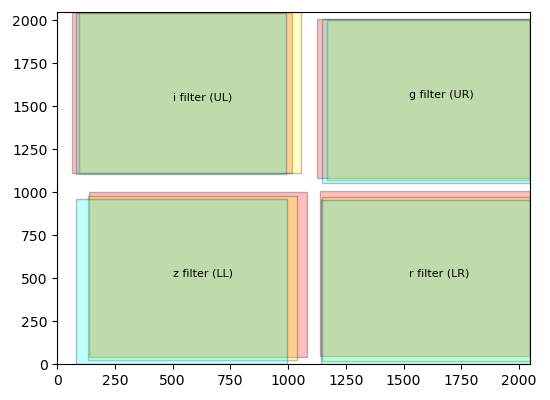
\includegraphics[scale=1]{images/showusedccd.png} \\
\end{center}   
\caption{This figure sets out the areas of the CCD used by the ROSS2
telescope which are used for the various filters at various times after
adjustment of the telescope. The area shaded in red is that prior to July 2015, the yellow shaded area is between
then and March 2019 and the blue part after then. The bulk of the area is
common to all of the configurations as can be seen. Note that all of the
{\rdwarf} observations, with which this report is concerned, start in 2017, well
after the first reconfiguration.} \protect\label{fig:showusedccd}
\end{figure}

Bias frames are taken daily for the visible light filters, usually 5 at
approximately 11:30 am and flat field frames nearly as often, usually 3 at a
time as the sky fades. A monthly master flat and bias file for each visible
light filter is also constructed from the daily flat and bias frames.

\subsection{Targets}
\protect\label{section:targets}

The three main targets of the Red Dots REM observations are \prox, {\bstar} and
\ross, all \rdwarf s.

\begin{description}
\item[\prox] is of spectral type M5.5 and at 1.30197 pc. is the nearest known
stellar object to the solar system. It is noted as having a significant flare activity, calculated
at 1.49 events per day in \citet{vida19} despite having a slow rotation period,
calculated at at 82.6 $\pm$ 0.1 days in \citet{collins17}.
\item[\bstar] is of spectral type M4 and at 1.8282 pc, is the fourth closest
stellar object to the solar system after {\prox} and Alpha Centauri A and B. Its
rotation period has been progressively given as 130 days in \citet{benedict98},
148.6 days in \citet{suarezmascareno15} and 145 $\pm$ 15 days in \citet{toledopadron18}.
Activity is low, as noted in the latter.
\item[\ross] is of spectral type M3.5 and at 2.976 pc, is the eleventh nearest
known stellar object to the solar system. Its strong activity is noted in
\citet{wargelin08}. As discussed in the draft paper included herewith, there is a wide variation in
some of the parameters for {\ross}, in particular the value of \vsini, the
radius and the rotation period. It became clear that an early benchmark of the work on the
{\rem} data would be clarification of the rotation period.
\end{description}

\subsection{Number of observations}
\protect\label{section:numobs}

The number of observations for each of the targets (and other objects used in
other projects) is given in Table \ref{table:numobs}. In Fig.
\ref{fig:rdwarfhist} is shown the distribution of observations of these targets
by date.

\begin{table}[!htbp]
\begin{center}
\begin{tabular}{lrr}
Target & Number of obs & \% \\
\hline
\prox & 36,312 & 17.16 \\
\bstar & 8,785 & 4.15 \\
\ross & 23,236 & 10.98 \\
Others & 143,329 & 67.72 \\
\hline
Total & 211,662 \\
\end{tabular}
\end{center}
\caption{This table shows the number of observations taken of each target
object, also showing the number of observations of other objects taken by other
projects. The number of usable observations of each target object is roughly
94\%
for the {\gfilter} and {\rfilter} cases, but significantly more for the
{\ifilter} and {\zfilter} cases.} \protect\label{table:numobs}
\end{table}

\begin{figure}[!htbp]
\begin{center}
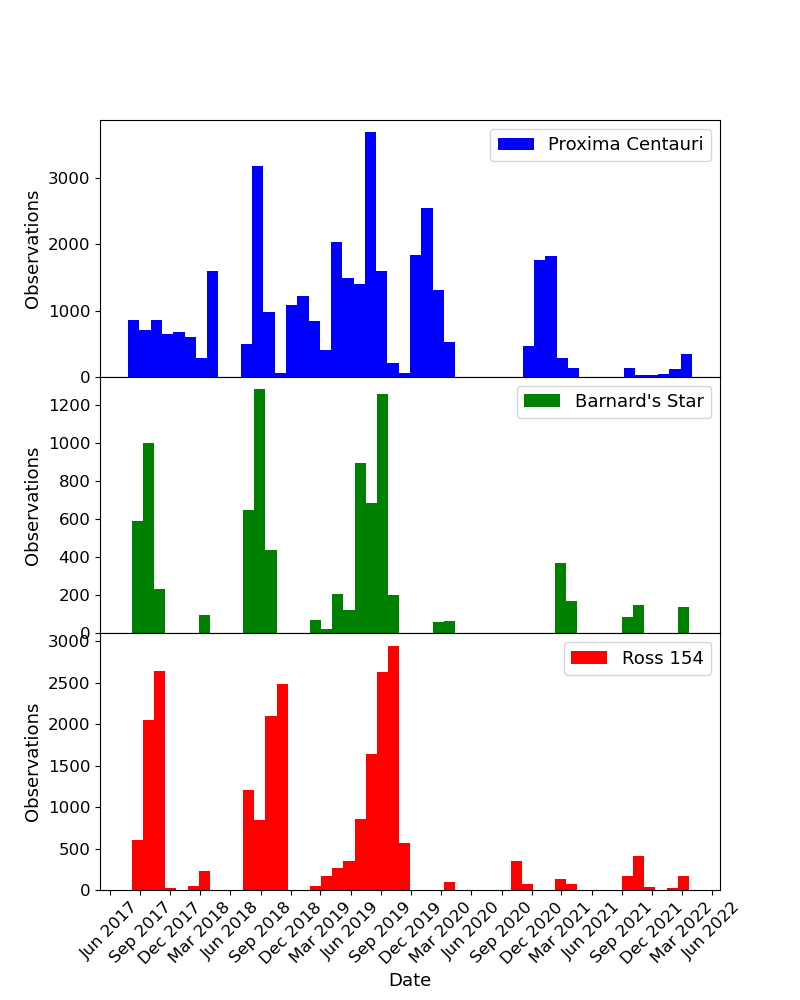
\includegraphics[scale=0.60]{images/rdwarfhist.png} \\
\end{center}   
\caption{This figure shows the distribution of observations of the three
{\rdwarf} targets to date, with {\prox} observations in the top pane, {\bstar}
in the middle pane and {\ross} in the bottom pane.}
\protect\label{fig:rdwarfhist}
\end{figure}

\subsection{Rotation periods and activity}
\protect\label{section:rotact}

The rotation period of each of the targets represents a most obvious
first objective of this study. As discussed in the draft paper, it is clear that
any surface features of the star, light or dark, cause a periodic signal to be
observed corresponding to the rotation period.

Rotation periods can give an indication of the age of the star, as discussed,
for example in the case of \ross, in \citet{wargelin08}. It has also been
noticed that a fast rotation period is correlated with strong activity. In
\citet{mohanty03} it is seen how activity increases, up to a limit, with a fast
rotation period. There have been various other studies, for example
\citet{aizawa22} and \citet{magaudda22} are recent papers in which rotation
periods and activity cycles are studied.

For this reason I decided to use detection of the rotation period as a benchmark
for analysis of the {\rem} data. The rotation period of {\ross} was somewhat
unclear in the literature and I made an effort to extract it from the data the
other literature referred to and then from the {\rem} data. Various figures for
the rotation period of {\bstar} exist and this is a clear target for further
study, however it should be noted that there are rather less observations of
\bstar, as noted in Section \ref{section:numobs}. Hopefully it may be possible
to obtain information about activity cycles and add to the correlation of this
with the rotation period.

\subsection{Proper Motions and caveats}
\protect\label{section:propermotions}
As all the target objects are amongst the closest objects outside the solar
system, they all have particularly large proper motions. Care must be taken to
track the proper motions of the targets and any adjacent objects.

The resolution of the ROSS2 camera is such that successive pixels
are approximately 0.6 arc-seconds apart (about 4.9 for Declination values, 6.9
for Right Ascension values but that varies a little with declination). This
means that proper motions of less than 20 milliarcseconds per year may be safely
disregarded which eliminates all but a handful of objects\footnote{18 objects
altogether, 10 in the vicinity of \prox, 1 in the vicinity of {\bstar} and 7 in
the vicinity of \ross.} in the vicinity of the targets from a need to track proper
motions for the bulk of other objects.

In Fig. \ref{fig:proxpm}, Fig. \ref{fig:bspm} and Fig. \ref{fig:rosspm} are
illustrated the proper motions \prox, {\bstar} and {\ross} respectively against
the immediate backgrounds.

\begin{figure}[!htbp]
\begin{center}
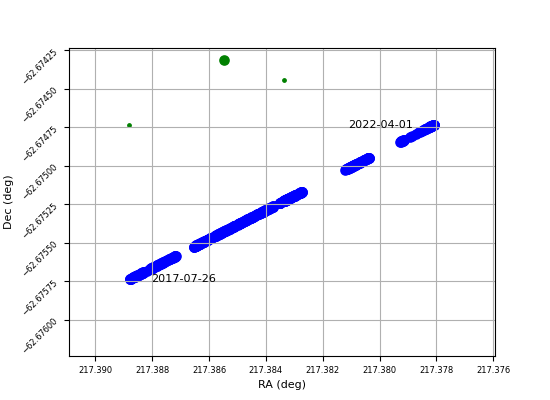
\includegraphics[scale=0.9]{images/pmprox.png} \\
\end{center}   
\caption{This figure tracks the proper motion of {\prox} against the immediate
background stars, showing start and end dates of the observations at the time
of writing, the gaps showing the periods where observations were not taken..} \protect\label{fig:proxpm}
\end{figure}

\begin{figure}[!htbp]
\begin{center}
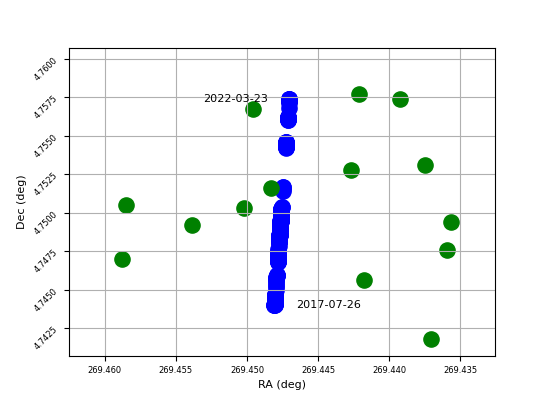
\includegraphics[scale=1]{images/pmbstar.png} \\
\end{center}   
\caption{This figure tracks the proper motion of {\bstar} against the immediate
background stars, showing start and end dates of the observations at the time
of writing, the gaps showing the periods where observations were not taken. The proper motion of {\bstar} is
extremely large and the scale is not the same as in Fig. \ref{fig:proxpm} or
Fig.  \ref{fig:rosspm} in consequence. Proper motion on Declination is so large
that the scale is reduced by a factor of 10 from that in Right Ascension.} \protect\label{fig:bspm}
\end{figure}

\begin{figure}[!htbp]
\begin{center}
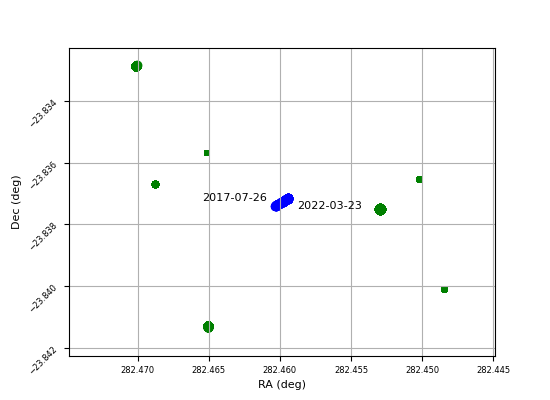
\includegraphics[scale=0.9]{images/pmross.png} \\
\end{center}   
\caption{This figure tracks the proper motion of {\ross} against the immediate
background stars, showing start and end dates of the observations at the time
of writing, the gaps showing the periods where observations were not taken.
The scale is the same as in Fig. \ref{fig:proxpm} (but not the same as in Fig. \ref{fig:bspm}).}
\protect\label{fig:rosspm}
\end{figure}

\clearpage

\section{Data provided by {\rem} observations}
\protect\label{section:tdataprovided}

\subsection{Data Available}

Consideration of the data available from the Red Dots project site is
hereinafter restricted to the targets of the project, the {\rdwarf} stars,
\prox, {\bstar} and \ross. The relevant data available is.

\begin{itemize}
\item Images taken with visible light filters \filtspec{g}, \filtspec{i},
\filtspec{r} and \filtspec{z} taken almost daily. although not necessarily of the {\rem} {\rdwarf} targets,
especially during April through to the first part of July each year when the position of the Sun in the sky makes
observations impossible. All the images of the {\rem} {\rdwarf} targets are taken
at a gain of 1 and the other targets with a gain of 4.4. 
\item Sky flat file images taken almost every day, usually as 3 images from the
sky, taken as the light fades. A set is taken with a gain of 4.4 and with a gain
of 1 each time, even if no observations are taken with that gain.
\item Bias file images taken each day
approximately 8 hours after the observations.
\item There are a very small number of dark file images (as for bias but with
an exposure of other than zero) taken in 2015, but these were from two years
before before the {\rdwarf} observations were commenced and are disregarded
herein.
\item Monthly master flat file images for each month constructed from some of
the daily flat files for the month in question.
\item Monthly master bias file images for each month, constructed from some of
the daily bias files for the month in question.
\item REMIR infrared images taken almost every day up to June 2019 and then
resumed in February 2021.
These are already reduced with the PREPROCESS software \citep{dipaola01}.
\item IDL routines used to prepare the master bias and flat files.
\end{itemize}

The flat and bias images are only available for the visible light filters
\filtspec{g}, \filtspec{i}, \filtspec{r} and \filtspec{z} as the REMIR images
have already been processed. Except in a small handful of cases dating back to 2015, two years
before the {\rdwarf} observations started, these and the observation files all
come as batches of four, one for each filter, all taken with the same exposure at the same time
and in the case of observations, looking at the same patch of sky.

The ROSS2 image files are stored with as 1024x1024 images, however the area of
the images is less than this as illustrated in Fig. \ref{fig:showusedccd}, the
upper and rightmost parts of the images are filled with zeros to make up to 1024
rows or columns. In all processing herein, the images are trimmed to the
appropriate size to avoid unnecessary computations with rows and columns of
zeros.

\subsection{Initial analysis of data}
\protect\label{section:initialanalysis}

The images are processed according to the formula:

\begin{center}
$ \frac{(mage - bias) \times mf}{flat - bias}$
\end{center}

In this $mf$ represents to mean value of the flat pixels. The master flat files
provided already have the bias subtracted.

\subsubsection{Some example image displays}
\protect\label{section:eximages}

In Fig. \ref{fig:initgexample} is illustrated a sample image from one of the
observations of {\bstar} using the {\gfilter}. In Fig.
\ref{fig:initgexample20} is shown a similar observation from March 2020. Note
how the second image is rotated clockwise by 90\degree{} from the previous image
and includes a different set of other objects for potential reference stars.

\begin{figure}[!htbp]
\begin{center}
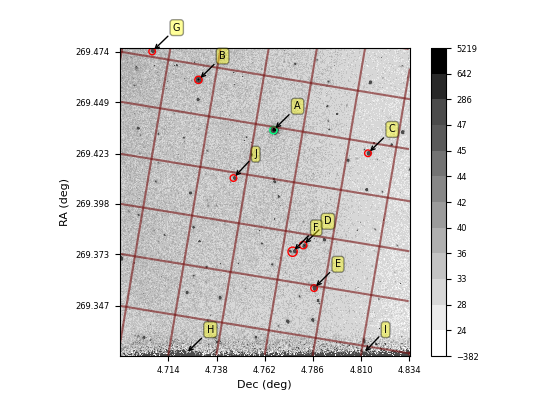
\includegraphics[scale=1]{images/initgexample.png}
\end{center}   
\caption{This is an observation of {\bstar} taken with the {\gfilter} on
17 September 2018 at 02:58:52 UTC after processing using the master bias and
flat files for September 2018. The brightest object, marked \textbf{A} and marked in
green is \bstar, whilst the next 9 brightest objects are marked in yellow and
\textbf{B}, \textbf{C}, etc. in decreasing order of brightness.}
\protect\label{fig:initgexample}
\end{figure}

\begin{figure}[!htbp]
\begin{center}
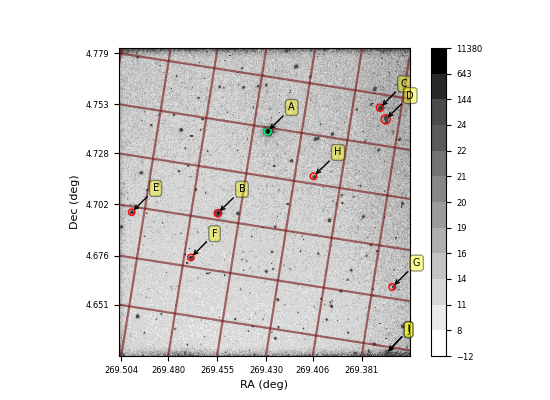
\includegraphics[scale=1]{images/initgexample20.png}
\end{center}   
\caption{This is an observation of {\bstar} taken with the {\gfilter} on
7 March 2020 at 09:07:23 UTC after processing using the master bias and
flat files for March 2020. The brightest object, marked \textbf{A} and marked in
green is \bstar, whilst the next 9 brightest objects are marked in yellow and
\textbf{B}, \textbf{C}, etc. in decreasing order of brightness.}
\protect\label{fig:initgexample20}
\end{figure}

In nearly every case there are 4 images taken, one with each of the 4 visible
light filters (in addition to the simultaneous REMIR observations) and in Fig.
\ref{fig:initgexample} is illustrated a set of observations of {\prox} taken on
the same date, 17 September 2018, as the observation of {\bstar} in Fig.
\ref{fig:initgexample}. For comparison, in Fig. \ref{fig:init4example20} is
shown a set of observations taken on 9 March 2020.

\begin{figure}[!htbp]
\begin{center}
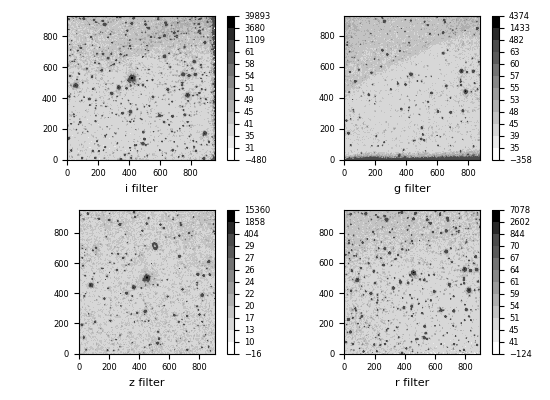
\includegraphics[scale=1]{images/init4example.png}
\end{center}   
\caption{This is all 4 observations of {\prox} taken with the visible light
filters on 17 September 2018 at 02:12:40 UTC after processing using
appropriate master bias and flat files for September 2018. They are arranged in
the order and orientation in which they are taken from the CCD. The
divisions on each image are pixel numbers.}
\protect\label{fig:init4example}
\end{figure}

\begin{figure}[!htbp]
\begin{center}
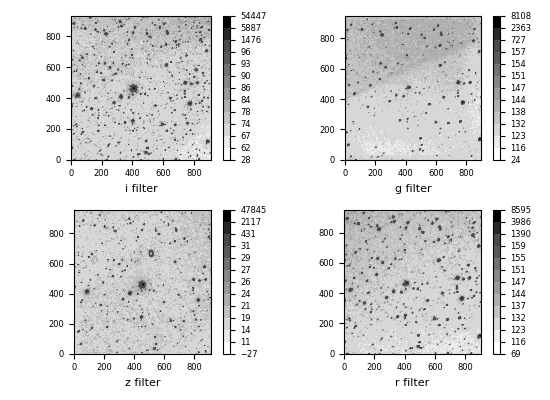
\includegraphics[scale=1]{images/init4example20.png}
\end{center}   
\caption{This is all 4 observations of {\prox} taken with the visible light
filters on 9 March 2020 at 08:56:14 UTC after processing using
appropriate master bias and flat files for March 2020. They are arranged in
the order and orientation in which they are taken from the CCD. The
divisions on each image are pixel numbers.}
\protect\label{fig:init4example20}
\end{figure}

\clearpage

\subsection{Caveats and matters to be addressed in analysing data}
\protect\label{section:mattersaddressed}

The following issues were apparent in the analysis of the data.

\begin{enumerate}
  \item There is no clear uncertainty measure in the master flat and bias files.
  \item The master flat files do not appear to be adequate, with some shading in
  	the images. This is particularly of concern with the {\gfilter}
  	towards the bottom part, although this is towards the centre of the CCD, as
  	shown in Fig. \ref{fig:showusedccd}.
  \item Some of the pixel values become negative after subtraction of the master
  	bias files.
  \item There is a ring-shaped artefact above and slightly to the right of the
  	brightest objects in the images for the {\zfilter}, invariably for
	the target, but to a greater or lesser degree for the other objects. Often the
	artefact lands entirely on another object, compromising the usability of the
	frame.
\end{enumerate}

As a result, it proved advisable to avoid the {\zfilter} as it would not
be practical to try to compensate for the artefact given the likely poor return
if this were done.


\section{Work done to date}
\protect\label{section:workdonetodate}

The following outlines the work done to date.

\subsection{Software tools}
\protect\label{section:softwaretools}

In order to manage the large number of files, I set up a database using MySQL
and a Python library and tool set to access this conveniently. The
\textit{Numpy}, \textit{Scipy} and \textit{Matplotlib} libraries were used
extensively. For some GUI tools, I used \textit{PyQt}. I also created an image
display tool which can display images and optionally save the images displayed
to file ready for incorporation in reports and papers such as this.

\subsubsection{Database and tools}
\protect\label{seciion:databaseandtools}

I set up a database and created a Python toolset to manage records of
each observation, the daily flat and bias files taken, records of objects in the vicinity of each target with
relevant data, where objects were found in the images and ADU calculation
results with uncertainties. Most relevant FITS files are stored in the database
but the toolset created transparently fetches other FITS files as required.

The toolset includes graphical tools to manage system parameters including
search criteria. In particular observation files, flat and bias records can be
selected using given criteria.

\subsubsection{Graphical display}
\protect\label{section:graphicdisplay}

The contrast on many of the images is poor and some of the standard image
display software, such \textit{AperturePT} and \textit{AstroImageJ} struggled
with several images. I wrote to the author of \textit{AperturePT} attaching some
of the images and he commented on the poor contrast.

I wrote a GUI program using \textit{PyQt} which enabled me to choose the
combination of grey scales which best highlighted the images. If an image is
loaded by the program, the effects can be seen in real time on the image. An
example of the dialog boxes is shown in Fig. \ref{fig:geditorshot}.

\begin{figure}[!htbp]
\begin{center}
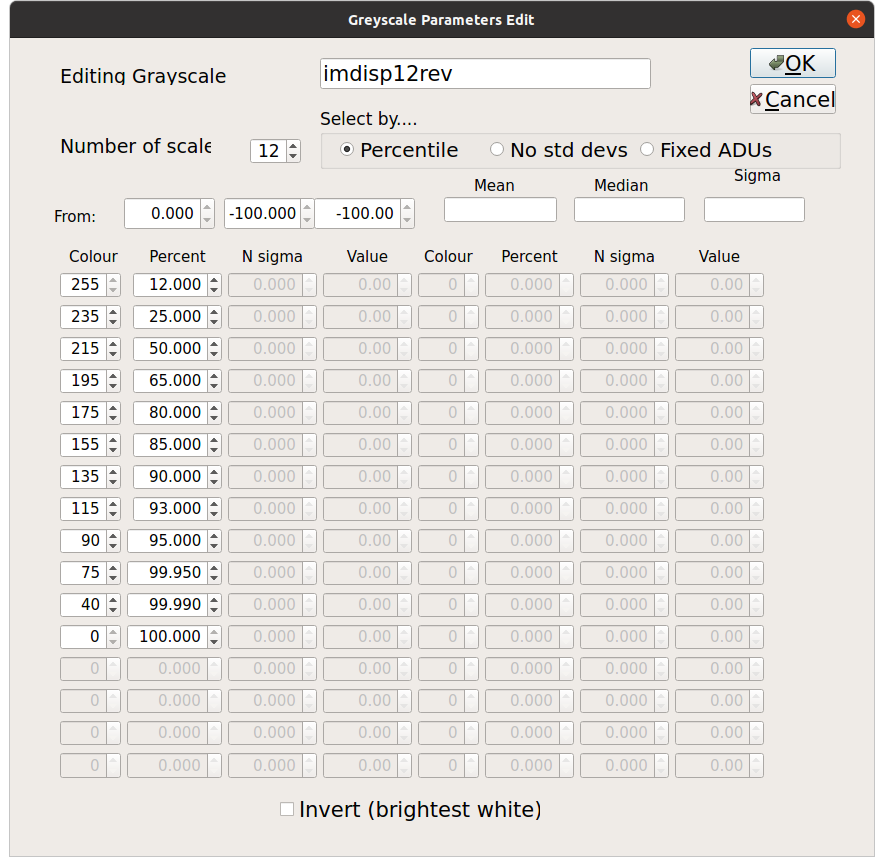
\includegraphics[scale=0.4]{images/geditorshot.png}
\end{center}   
\caption{This illustrates one of the dialogs from the graphical display editor
showing how the grey scales are tuned. Grey scales are assigned using
percentiles of the ADU values (default) by number of standard deviations or
absolute value. The values used are as shown in the figures. If an images is
loaded the other boxes are filled in to show the values from the current image
and updated, along with the figure displayed to show the effect on the image.
The results are saved in a configuration file for future use.}
\protect\label{fig:geditorshot}
\end{figure}

\subsection{Analysis of supplied master calibration files}
\protect\label{section:masterbiasflat}

In order to address the matters such as those referred to in Section
\ref{section:mattersaddressed} above, a study was made of the master bias and
flat files supplied.

The following problems were observed with these files.

\begin{enumerate}
  \item The number of daily bias or flat files going to make up the master files
  is not consistent, month by month. Each master file is made up entirely from
  the daily files for the calendar month concerned, which may vary considerably
  in number and criteria for selection. In Fig. \ref{fig:mastmeanbias} is shown
  the mean value and standard deviation of the master bias files up to March
  2020, showing the net effect.
  \item Some of the criteria for selection of the files, particularly the flat
  files, are unusual and unexplained.\footnote{The selection of the daily flat
  files is restricted to those for which the skewness is negative and the
  kurtosis is less than 7.}
  \item Some of the statistics for selection of daily files, notably the flat
  files are incorrectly calculated.\footnote{It did not seem a productive use of
  time to reproduce the programming error and work out the actual but incorrect
  set of daily flat files which went to make up the master flat files.}
  \item The master bias files, as constructed, include some extreme values for
  some pixels which cause values for the image files to go negative when the
  bias file is subtracted. No account is taken of noisy or unreliable pixels.
  \item The daily flat files consist of sets of 3 in decreasing light and the
  median value is taken, the result being then normalised. This causes the
  benefit of the brighter flat files, with their better signal to noise ratio to
  be ignored in addition to the other ones.
\end{enumerate}

\begin{figure}[!htbp]
\begin{center}
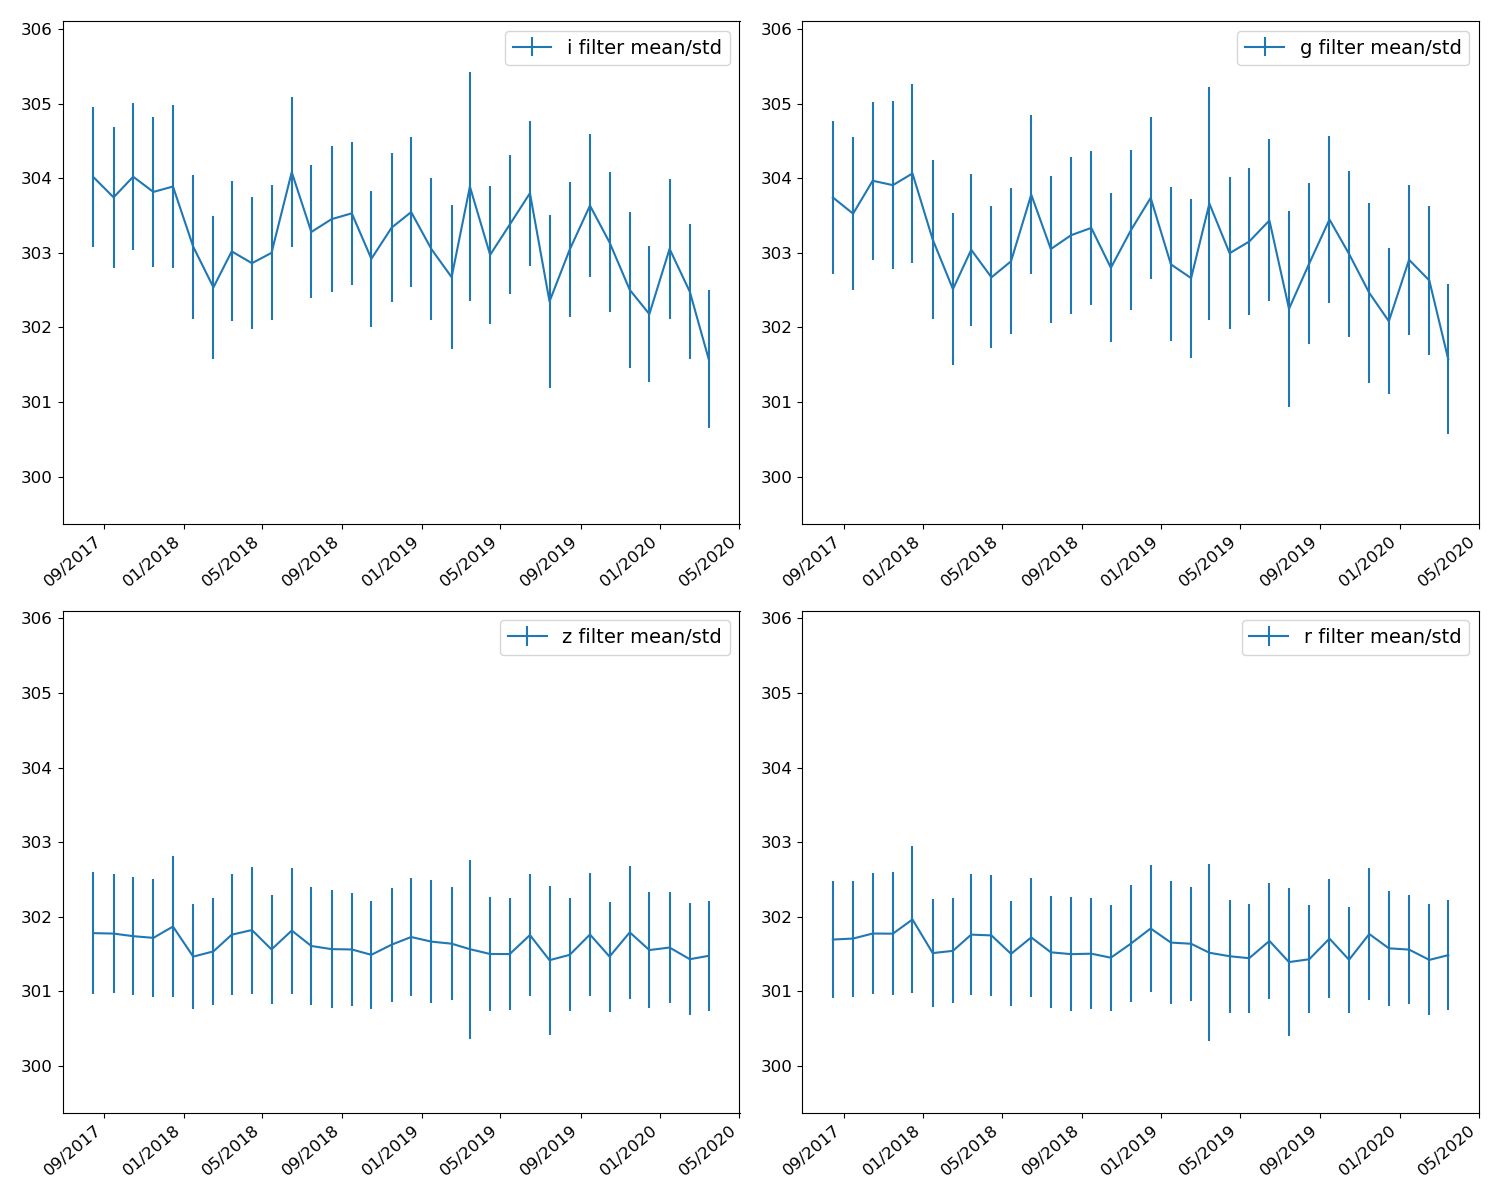
\includegraphics[scale=0.4]{images/mastmeanbias.png}
\end{center}   
\caption{This illustrates the mean and the standard deviation of the values in
the master bias files from July 2017, when {\rdwarf} targets were first
observed, until March 2020.}
\protect\label{fig:mastmeanbias}
\end{figure}
\clearpage

\subsection{Construction of alternative master bias and flat files}
\protect\label{section:altcalib}

Having considered and tried to use the supplied master bias and flat files, I
decided to construct alternative ones from the daily bias and flat files
provided.

A key element in this was to construct the files using a rolling ``window'' of
the same number of daily files centred on the relevant date. This made a
substantial difference to the resulting master files, all of the variations
seen in Fig. \ref{fig:mastmeanbias} from month to month were eliminated and the
resulting files were very similar.

\subsubsection{Defective or unreliable pixels}
\protect\label{section:badpix}

I undertook a study of all the files, flat files, bias files and observation
files to determine whether any pixels in the CCD array could be counted as
``bad'' or unresponsive, had particularly high mean values or large standard
deviation. The literature varies somewhat on how bad pixels are defined or
determined.

\Notnow{Of recent papers, \citet{allers20} define bad pixels as ``dead'' pixels or pixels
with an uncertainty in the flat fields of over 10\%. In \citet{piskunov20} bad
columns in the CCD used are first identified and eliminated and then an
iterative procedure is adopted to effectively assign weights to each pixel. In
\citet{bongiovanni19} a procedure based on constructing two composite flat
fields from low and high counts and regarding as bad the pixels where the ratios
differ by more than 15\%. In \citet{belli18} a bad pixel mask is constructed by
selecting pixels in the flat fields with very low counts and those in the dark
frames with very high counts (but the criteria for ``low'' and ``high'' counts
in those files are not defined). In \citet{briesemeister18} pixels in the
constructed flat fields with values less than 0.5 or greater than 1.5 are
considered to be bad.

A comprehensive study of the quality of pixels is described in the
recently-published \citet{maslennikova20}. Pixels are described as
\textbf{Normal}, \textbf{Cold}. \textbf{Warm}. \textbf{Dead}, \textbf{Hot} and
\textbf{Inverse} according to the responses. The pixels on the ROSS2 telescope
CCD do not fit neatly into these brackets, apart from the \textbf{Normal} ones.}

For the purposes of this study, it was clear that the pixels could be described
as:
\begin{description}
\item[Normal] pixels are those which are clearly well-behaved with a linear
response within 10\% of saturation.
\item[Consistently high] pixels are those which whose count never falls below a
value significantly higher than bulk of the pixels. These are often found in
whole sections of a column on an array.
\item[Noisy] pixels are closest to \textbf{Dead} pixels as defined in 
\citet{maslennikova20}. Included are those with consistent high levels of noise,
with the standard deviation on the bias level over 5 times the standard
deviation.
\item[Bad] pixels are ones which give random readings, usually very low ones.
\end{description}

In addition, all of the pixels, to a greater or lesser extent, can give random
very high readings which stand out from the neighbouring pixels. These might
perhaps be due to cosmics in some cases, or because on resetting the CCD those
pixels are not reset. Some are random much more often than others and these
correspond to the \textbf{noisy} pixels.

There are very few examples, in the order of 25 pixels spread over the used area
of the array, which qualify as \textbf{bad}.

It is straightforward to interpolate over the relevant pixels. There are a few places where there are strings of
adjacent noisy or consistently high pixels, but these almost entirely affect
columns in the CCD, the worst example can be found in the area used for the \gfilter, seemingly as
the CCD is read out by columns, so adjacent pixels on the same row have to be
used for interpolation.

\subsubsection{New master flat and bias files}
\protect\label{section:newmastfb}

With appropriate adjustments for the defective pixels as described above, it
proved straightforward to construct new master bias files using a  ``rolling
window'' centred on the date required. I constructed standard deviations for each individual pixel.

I made an extensive study of the linearity using the daily flat
files; it would  appear than the performance is linear up to 62,000 counts per
pixel out of a possible 65,536. I constructed the master
flat files using daily files with pixels between a range of 5,000 and 61,000 to be clear of this linearity cut-off.
None of the image files, other than ones contaminated by cosmics and similar,
had pixel values close to 60,000. I did not use the skewness or kurtosis
measurements used in the construction of the original master flat files as this
did not seem to have any benefit\footnote{Even if they were correctly
calculated.}. I then subtracted from the selected daily flat files
the newly-constructed master bias file centred on the relevant date and normalised the result.
I then combined the results into a master flat file for the relevant date using a weighted geometric mean,
the weights being inversely proportional to the standard deviations.

This resulted in a much more satisfactory set of master bias and flat files and
it was possible to much more confident of the uncertainty of values on a
per-pixel basis. The combination of the flat files using a weighted
geometric mean, included many more of the brighter files, with their higher
SNR, giving them priority over the darkest files, whilst still obtaining some
benefit from the latter.

When the object ADU counts from {\rem} images are computed from the images, the
standard deviations for each individual pixel in the image are combined into an
overall standard deviation for the ADU count for the relevant object.

\subsection{Finding and identifying objects}
\protect\label{section:findingidentify}

Most of the objects in the neighbourhood of the target {\rdwarf} objects were
identified using GAIA DR3. Where alternative shorter names than GAIA DR3 nnnnnnn
were found, this was used in preference. Bearing in mind the resolution of the
{\rem} telescope of around 0.6 arcsecond, objects closer together than this
distance were eliminated, as were objects with irregular profiles and one marked
as variable.

The magnitudes in various bands are all noted in the database records, but these
were mainly used as a guideline where there was ambiguity in distinguishing
close but not overlapping objects. It proved better to explicitly count the ADUs
after adjusting the aperture sizes.

There remains considerable work in finalising the optimal aperture sizes for
each objects, particularly with {\prox} and {\bstar}.

The best frames contain up to 200 possible reference stars for the best
examples, more for {\prox} and less for {\bstar}. Average frames contain up to
30 or so. Any less than 10 are rejected as too poor in contrast, but the total of rejected frames is less than
10\%.\footnote{This figure is subject to amendment, currently the rejection is
binary, but there is provision for a ``quality'' marker enabling frames to be
partially used where appropriate.}

\subsection{Calibration of reference stars and ADU counts}
\protect\label{section:calibrationrefstars}

Not all the frames contain the same reference stars, or have the same
orientation, some are rotated by 90\degree or 180\degree relative to others. The
target object may be off-centre by varying amounts and in varying directions and
different reference objects appear in different frames, or are too close to the
edge in some cases, where vignetting or similar reduces the accuracy, to be
usable. Only quite a small handful of objects appear in all the frames.

After some experimentation with strategies for computing and calibration of the
objects, the most promising strategy emerged as being for each filter
(initially this was only done with the {\rfilter} images, being the least
problematic).

\begin{enumerate}
  \item Compute the ADU count and standard deviation for each object in each
  frame.
  \item Compute the mean ADU count and corresponding standard
  deviation for each object. Clearly strongly variable objects previously missed can be weeded out
  at this stage.
  \item For each observation, perform a linear regression fit of the calculated
  ADUs for each object other than the target in the frame to the mean ADUs.
  \item Apply the fit backwards, propagating the standard deviation, to the
  calculated ADUs for the target on the frame and compare with the mean ADUs for
  the target to give the variation from the mean of the target for that frame.
\end{enumerate}

This technique proved very successful, in most cases the correlation of the
linear regression was better than 95\%, and proved insensitive to what set of
reference stars were available on a particular frame.

\subsection{Results for \ross}
\protect\label{section:resultsross}

The results for {\ross} are set out in the draft paper attached to this report.
but in summary the data sources referred to in papers which mentioned
measurements for {\ross} were studied and a rotation period of $2.87 \pm 0.01$
days was confirmed consistently.

After processing the data using the modified bias and flat files and processing
the counts relative to the reference stars as described above in Section
\ref{section:calibrationrefstars}, the period of 2.87 days was clearly extracted
from the data.

This confirms that there is viability in the methods used in terms of recovering
the rotation period for \ross. More challenging may be that for \bstar, where
the number of observations is less and also the number of reference objects.

\subsection{Set up of pipeline}
\protect\label{section:pipeline}

A daily routine was set up to interrogate the {\rem} results and load new data
into the database. The steps were:

\begin{enumerate}
  \item Load information about new observations into the database. This is just
  a simple record of information.
  \item Load FITS files corresponding to the ROSS2 observations of the target
  objects into the database cache.
  \item For loaded FITS files, add data about statistics such as maximum and
  minimum pixel values, mean and standard deviations into the database.
  \item For database rows corresponding to the targets, compute the barycentric
  dates and add to the database.
  \item Identify the target and other objects in the frames and add locations to
  the database. Mark frame as too poor to use if the target is not found, and
  less than a given number of reference objects, currently 10, are not found.
  \item Load FITS files corresponding to daily flat and bias files into the
  database.
  \item Load any new master bias and flat files (although these are no longer
  used).
\end{enumerate}

The calculation of ADUs for objects is currently done manually when ready, but
ultimately this will be added to the pipeline. Currently the daily job takes
about 40 minutes to run.

%\input{rossper.tex}
%\input{processing.tex}
%\input{results.tex}
\section{Further work following progression}
\protect\label{section:worktocome}

The following is the programme of work I need to undertake in order to regard
the project as complete.

In a lot of cases, the work already done will need revisiting and refining and
``iterating until convergence'' achieved.

I see the following as necessary, not in any particular order.

\begin{enumerate}
  \item Better handle bad or unreliable pixels identifying ones prone to
  ``spikes'' and bouts of insensitivity and improving the interpolation over
  them. Where they land on an object, it would be better to interpolate using
  any fitted Gaussian profile.
  \item Optimise as many as possible of the reference object apertures and
  identify irregularly shaped and variable objects.
  \item Look at other filters, such as the \gfilter, possibly the other filters,
  although the number of available reference objects looks poor and the
  {\zfilter} images all have artefacts in them.
  \item Repeat the work done for {\ross} with {\prox} and {\bstar} and consider
  periodograms for them.
  \item Extend the work done to date to the REMIR near infrared images.
\end{enumerate}

\section{Accuracy}
\protect\label{section:accuracy}

It seemed worth looking at whether any adjustments of the exposure times might
improve the accuracy, as many of the objects which might be used for reference
give an ADU count only just above the sky level. The exposure times currently
are 10 seconds for {\prox} and {\ross} and 5 seconds for \bstar.

Table \ref{table:pixvals} is set out the maximum value in any of the observation
files for each target and each filter and the percentage of observation files in
which at least one pixel exceeds a give number of ADUs (this does not currently
take account of defective pixels or cosmics, but these would have negligible
effects on the results).

It is clear that some increase in exposure time, possibly up to 5 times or more
in the case of the \gfilter, would benefit the contrast, except
for the {\ifilter} results, which are generally too close to saturation.
The nature of the instrument, however, may not permit any different exposure
times to be made with different filters.

\begin{table}[!htbp]
\begin{center}
\begin{tabular}{|l|r|rrrr|} \hline
Filter & Max value & \% over 30,000 & \% over 40,000 & \% over 50,000 & \% over
60,000 \\\hline
 \multicolumn{6}{|c|}{\textbf{\bstar} exp 5 sec} \\\hline
\texttt{g} & 63,422 & 0.05 & 0.05 & 0.05 & 0.05 \\
\texttt{i} & 63,448 & 78.94 & 61.15 & 45.71 & 0.77 \\
\texttt{r} & 54,806 & 16.68 & 3.73 & 0.97 & 0.00 \\
\texttt{z} & 63,387 & 12.52 & 3.37 & 0.87 & 0.05 \\
\hline
\multicolumn{6}{|c|}{\textbf{\prox} exp 10 sec} \\\hline
\texttt{g} & 63,466 & 0.38 & 0.30 & 0.25 & 0.18 \\
\texttt{i} & 63,457 & 74.15 & 52.88 & 36.84 & 4.03 \\
\texttt{r} & 63,425 & 0.60 & 0.10 & 0.09 & 0.08 \\
\texttt{z} & 63,456 & 25.38 & 11.64 & 5.47 & 0.16 \\
\hline
\multicolumn{6}{|c|}{\textbf{Ross 154} exp 10 sec} \\\hline
\texttt{g} & 63,453 & 0.41 & 0.35 & 0.28 & 0.22 \\
\texttt{i} & 63,452 & 76.71 & 57.35 & 39.25 & 2.16 \\
\texttt{r} & 63,268 & 7.99 & 2.38 & 0.93 & 0.11 \\
\texttt{z} & 63,447 & 8.33 & 2.14 & 0.45 & 0.04 \\
\hline
\hline
\end{tabular}
\end{center}
\caption{This figures shows the maximum ADU values of any pixel in any of the
observation files for each of the 3 {\rdwarf} targets for each filter. The
following columns show the percentage of pixels in each case which are above
30,000, 40,000, 50,000 and 60,000.}.
\protect\label{table:pixvals}
\end{table}
\clearpage

%\input{database.tex}

\bibliographystyle{apj}
\bibpunct{(}{)}{;}{s}{,}{,}
\bibliography{bibrefs}

\protect\label{lastpage}
\end{document}
